\chapter{Introduction}
\label{intro}

High performance machines are increasingly using GPUs~\cite{15, 16, 17, 18, 19}, to leverage their scalability and low dollar to FLOPS ratios.  As a result, GPUs have become the main compute engines for today’s HPC clusters and supercomputers like the Titan supercomputer in Oak Ridge~\cite{titan}. This trend continues with the move toward exascale machines~\cite{exascale1, exascale2, exascale3, exascale4, exascale5, exascale6, exascale7}, with compute nodes expected to be comprised of millions of accelerator and general purpose cores, whether packaged as `thin' or `fat' nodes (shown in Figure~\ref{fig:hybrid}).  Therefore, it is not only important to efficiently schedule applications to keep all the available cores busy but also  intelligently move the appropriate data near the computation as these accelerators have limited amount of memory attached to them. Existing software infrastructures deal very poorly in terms of scheduling and fine grain resource management of such heterogeneous architecture leading to substantial underutilization of all the available resources, including both the computational and data movement engines. Next we describe three broad classes of applications where there is substantial GPU underutilization and showcase the current scheduling crisis in them. 

\begin{figure}[h]
\begin{center}
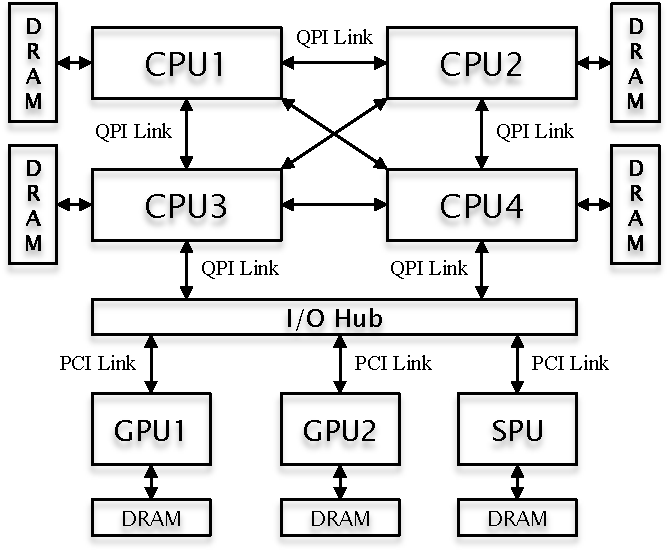
\includegraphics[width=0.70\textwidth]{hybrid}
\caption{Accelerator-based heterogeneous system architecture }
\label{fig:hybrid}
\end{center}	
\end{figure}

\begin{figure}[t]
\begin{center}
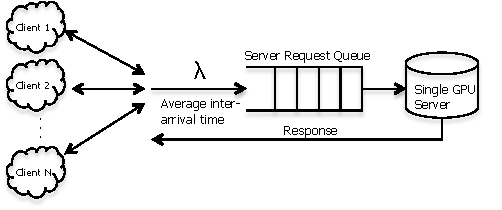
\includegraphics[width=0.70\textwidth]{servicemodel}
\caption{GPGPU application service model following a negative exponential
distribution of request arrival from multiple end users. }
\label{fig:service}
\end{center}	
\end{figure}

\section{GPU Sharing in Cloud}
A recent trend is the gain in popularity of computationally intensive high performance applications in client-server workloads including image processing algorithms like video transcoding~\cite{element} , financial algorithms~\cite{zillians}, online gaming, e.g., NVIDIA’s cloud gaming~\cite{nvidia-game}, search~\cite{GPUsearch}, data mining~\cite{GPUmine} and multimedia services like Adobe’s Photoshop.com~\cite{adobe}. This motivates online services to take advantages of GPU clusters. This is mirrored by GPU offerings by cloud providers like Amazon ECC~\cite{amazon}, Nimbix~\cite{nimbix}, Peer1 Hosting~\cite{peer1}, and Penguin Computing~\cite{penguin}.  Figure~\ref{fig:service} shows the application service model for a multi-tenant single GPU server.

A challenge to using GPUs in these multi-tenant server and cloud environment is the lack of sophisticated support for GPU scheduling, given the predominant model of treating GPUs as statically chosen devices, in which applications explicitly and programmatically select the GPU devices on which they wish to run, rather than as first class schedulable entities~\cite{pegasus}. Such static GPU assignments will inhibit concurrency, particularly with the varying workloads imposed by web applications. For instance, during peak demands for certain services, some GPU devices will be heavily utilized while other services’ GPUs will be idle or underutilized. Low GPU utilization can also be attributed to considerable diversity in the fraction of CPU vs. GPU component in applications, for reasons that include an inability to parallelize certain application components and/or limited GPU residency vs. the costs of host-GPU data transfers. Finally, although each GPU can internally contain thousands of cores, it is treated by applications as a single SIMD engine, potentially resulting in the serial execution of GPU contexts that could have been executed concurrently.

\section{Large-Scale Graph Analytics on GPUs}
With the increasing interest in many emerging domains such as social networks, the World Wide Web (e-commerce and advertising), and genomics, the importance of graph processing has grown substantially. Some examples of graph analytics include friend/product recommendations, anomaly and trend detection, online advertisement serving etc. This recent trend has given rise to many graph processing frameworks in both distributed, e.g. GraphLab~\cite{graphlab}, PowerGraph~\cite{powergraph},  Pregel~\cite{pregel}; and single machine shared-memory environments, e.g.  Graphchi~\cite{chi}, X-Stream~\cite{xstream}, Ligra~\cite{ligra} etc. This need to rapidly process large graph-structured data has also engendered recent efforts to leverage cost-efficient GPUs for efficient graph analytics. Doing so, however, requires addressing substantial technical challenges, including (1) dealing with the dynamic nature of graph parallelism, (2) coping with constrained on-GPU memory capacity, i.e., to process graphs with memory footprints that exceed that capacity, and (3) addressing programmability issues for developers with limited insights into how to best exploit the resources of evolving and varied GPU architectures.

More precisely, a graph processing framework using GPUs should expose abstractions or simple APIs for the developers to write the appropriate sequential codes for their domain specific algorithms, e.g., for data mining, machine learning, etc to express their use for processing graphs of arbitrary size. The runtime should then seamlessly (i) partition the graphs into smaller chunks each single one of which entirely fits into GPU memory, (ii) efficiently move data between host and device leveraging concurrent GPU operations to obtain fine-grain parallelism that exploits both GPU software and hardware features like CUDA streams and Hyper-Q of Kepler GPUs etc (iii) choosing the most appropriate programming model ( edge- or vertex- centric or a combination of both) to generate device code for efficient GPU-level graph processing, and iv) finally intelligent coordinated scheduling and management of both the data movement and compute engines to achieve optimal performance. With such automation, we can deal with graph sizes much exceeding GPU memory sizes. This is important because even a common Yahoo web-graph comprised of 1.4 billion vertices requires approximately 6.6 GB of memory to store just its vertex values (not even including the edges and their corresponding states).

In summary, the goal is to  design a scale-up graph processing framework on HPC systems with discrete GPUs and high end (i.e., memory-rich) hosts where GPUs can be used to accelerate analytics performed on graphs with billions of edges, operating at speeds much exceeding that of similar operations run on CPUs, and programmed in ways accessible to programmers who are not experts in GPU programming. 

\begin{figure}[t]
\begin{center}
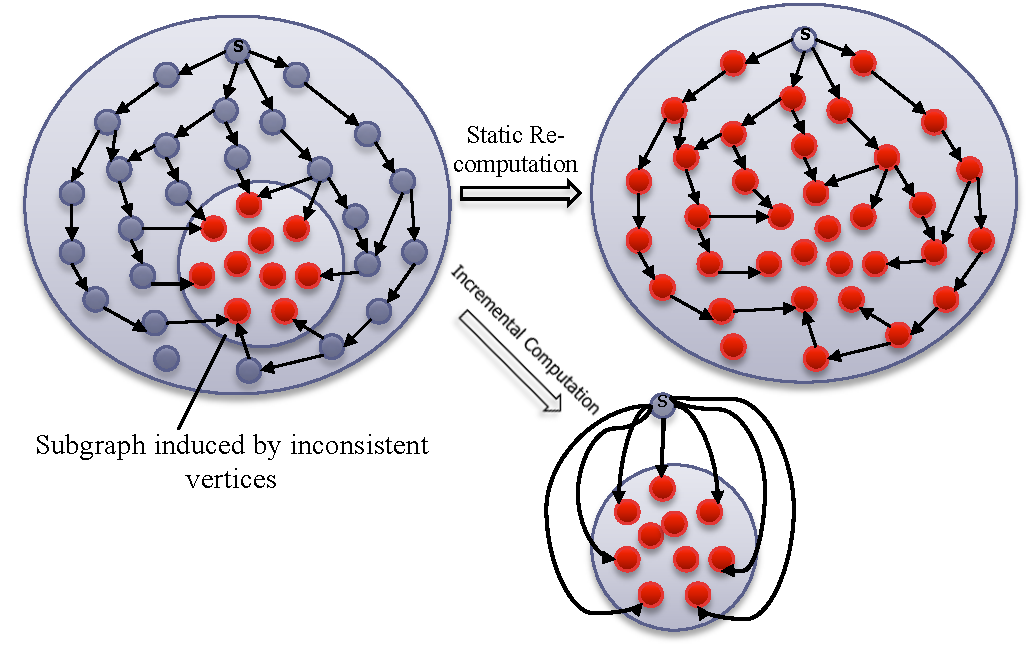
\includegraphics[width=0.70\textwidth]{incremental-graph}
\caption{Static vs. incremental graph processing. }
\label{fig:inc}
\end{center}	
\end{figure}

\section{Dynamic Graph Analytics on GPUs}
Another important aspect of real-world graphs like facebook friend lists or twitter follower graphs is that they dynamically change with time.  Current graph analytics on such dynamic graphs follow a store-and-static-compute model that involves first storing batches of updates to a graph applied at different points in time and then repeatedly running static graph computations on multiple versions or snapshots of this evolving graph sequence. The key assumption made here is that the rate of change in graphs due to continuous updates is slower than the execution time of the static graph analytics. This assumption might not hold true for current real-world graphs. For instance, Twitter traffic can peak at 143 thousand tweets (and associated updates) / per second and emails sent per second can reach as high as 2.5 millions/sec.   Hence, there are two fundamental challenges to applying static recomputation to these types of rapidly changing data sets. First, static graph analytics on a single version of the evolving graph, even when leveraging massive amount of parallelism offered by multiple cores in a high performance cluster, can be very slow due to the extreme scale of many real-world graphs and/or because of the complexity of the graph queries that are traditionally both compute and memory intensive. Therefore, the cumulative cost of analyzing such large-scale versions with complex graph queries repeatedly can be substantially high. Second, there are real world graph analytics problems that inherently require soft or hard real time guarantees, e.g., real-time anomaly detection, disease spreading etc. So to conclude, the current high volume and velocity of graph data combined with the complexity of user queries has outstripped the traditional static graph analytics model on streaming graphs.

To address the above mentioned computational crisis in dynamic graph processing we need a graph processing framework that can incrementally process a continuous stream of updates (i.e., edge/vertex insertions and deletions) as a sequence of batches.  Because the incremental logic, in many practical scenarios, affects only a portion of the graph (as shown in Figure~\ref{fig:inc}), this reduction can result in tremendous performance benefit compared to static recomputation of the graph algorithm on the entire graph for many popular graph algorithms and real-world graphs.
Further, we also need to handle the scenarios when updates to the graph affects a very large portion of the graph and incremental processing won’t help much or may even be worse (due to overheads of incremental execution)  compared to a static recomputation. E.g., in incremental BFS, updates that affect vertices close to the root node affect nearly the entire BFS tree. In this case, the incremental run can at best perform as good as the static re-run.  Hence a characterization of graph algorithm that would benefit the most from incremental processing is essential. Finally, in order to allow faster updates to the graph and run both the incremental and static graph algorithms efficiently on GPUs, we need to design appropriate data structures specifically tailored to store both the graph and the updates for  efficient scheduling and data movement between the host and the device. 

\section{Thesis Statement}
\label{thesis}
The future exascale machines with compute nodes are expected to be comprised of millions of heterogeneous accelerator-based and general purpose cores. It is a huge challenge to efficiently schedule applications and place the appropriate data near the computation. To address this resource management and scheduling crisis we must build system-level design and abstractions that support load balanced scheduling of application requests to avoid request collisions, feedback-based mechanisms for efficient data movement and placement, system-level support for reducing core idling and seamlessly scaling to large input datasets for out-of-core processing to achieve optimal performance in a wide variety of applications.   

\section{Contributions}
The key contribution of our research is a set of technologies that addresses the aforementioned challenges. Specifically, to validate the thesis, we make the following contributions:
\begin{itemize}
\item \textbf{Strings Scheduler.} To address the challenges in scheduling multi-tenant cloud workloads in the heterogeneous resources of future, high-end manycore GPU-based server platforms we design and implement the Strings scheduler, a two-level hierarchical scheduler that decomposes the scheduling problem into a combination of load balancing and per-device resource sharing. The workload balancing intelligently binds each application’s GPU component to an appropriate GPU and the device-level, per-GPU scheduler handles GPU resource sharing for the multiple tenants mapped to a single GPU, to improve application performance while also meeting system-level goals like high throughput, fairness, etc. It implements a model in which accelerators like GPUs are first class schedulable entities rather than statically chosen devices used as single SIMD engines. The intent is to avoid the serial execution of GPU contexts that could otherwise have been executed concurrently, as with the varying workloads imposed by web applications, where during peak demands, the current model of static GPU assignments will cause some GPU devices to be heavily utilized while others are idle or underutilized. Explicit scheduling can also avoid underutilization caused by the differences in the fraction of CPU vs. GPU components seen across different applications, for reasons that include an inability to parallelize certain application components and/or limited GPU residency vs. the costs of host-GPU data transfers. Strings makes GPUs into explicitly scheduled entities by overriding the device selection calls made by applications. It then manages these calls with the aforementioned two-level scheduler, at the top, balancing workloads across the multiple GPUs resident in each manycore node, and at the device level, reducing GPU core idling via GPU multi-tenancy and the judicious overlap of GPU execution with host-GPU data movements. Strings also supports true GPU multi-tenancy, termed the `Context Packing', which dynamically packs the GPU contexts of multiple applications into a single context, to achieve high GPU utilization and low context switching overhead. Additional methods enable in providing dynamic feedback from device-level schedulers to workload balancer, to inform the global decisions made by the latter about characteristics of the applications being scheduled by the former.

%Strings makes it easy to experiment with and evaluate alternative scheduling strategies for future heterogeneous manycore platforms. In this thesis, using workloads drawn from diverse classes of GPGPU applications, experimental results obtained with Strings are obtained for three different workload balancing strategies, three GPU scheduling policies, and four feedback policies. GPU scheduling policies presented and evaluated using Strings are distinct from prior work in their explicit consideration of data movement to/from the GPU device. The Phase Selection (PS) policy, which maximizes GPU utilization by smartly selecting and co-scheduling applications that currently operate in different phases computation vs. communication - of their combined CPU/GPU execution. Advanced feedback-based policies, termed Data Transfer Feedback (DTF) and Memory Bandwidth Feedback (MBF), that exploits the advantages offered by CUDA streams by collocating applications with contrasting behavior, in terms of data transfer and memory intensity, to achieve extreme performance benefits.

\item \textbf{GraphReduce Framework.} To address the problem of processing graph applications with larger memory footprint than the device memory, we present GraphReduce (GR), a highly efficient and scalable GPU-based  out-of-core graph processing framework that operates on graphs that exceed the device’s internal memory capacity. GraphReduce supports an access pattern based hybrid computational model adopting a combination of edge- and vertex-centric implementations of the Gather-Apply-Scatter (GAS) programming model to match the different types of parallelism present in different phases of the GAS execution model. GR achieves efficiency in graph processing via improved asynchrony in computation and communication (operating on multiple asynchronous GPU streams), by dynamic characterization of data buffers based on data access pattern and access locality to fully exploit the high degrees of parallelism in GPUs.   Additional hardware parallelism is extracted via \textit{spray streams} for deep copy operations on separate CUDA streams. GR runtime also uses computational frontier information for efficient GPU hardware thread scheduling and data movement between host and GPU. Specifically, GR moves data into GPU memory only when a subset of the graph has at least one active vertex or edge. Further, when possible, GR uses dynamic phase fusion/elimination to merge/eliminate multiple GAS phases, to avoid unnecessary kernel launches and associated data movement.

\item \textbf{EvoGraph.} Because of the extreme scale of real-world graphs and the high rate at which they evolve combined with the complexity of user queries, traditional processing methods by first storing the updates and then repeatedly running static graph analytics on a sequence of snapshots are deemed undesirable and computational infeasible on GPUs. To address such challenges of processing real-world graphs that are constantly evolving over time we present the design and implementation of EvoGraph, a high performance dynamic graph analytics framework for evolving graph analytics on GPUs that incrementally processes graphs on-the-fly using fixed-sized batches of updates.    As part of GraphIn, we propose a novel programming model called I-GAS that is based on the gather-apply-scatter programming paradigm and that allows for implementing a large set of incremental graph processing algorithms seamlessly across multiple GPU cores.  We further propose novel optimizations like property-based dual path execution in the EvoGraph framework to choose between an incremental vs static run over a particular update batch and GPU 'context merging' to merge and collocate the GPU contexts of static and incremental graph algorithms on the same GPU, inorder to avoid context switching overhead and efficiently use of all hardware resources using GPU streams, including its computational and data movement engines.

\item An extensive performance evaluation of each of the above runtime frameworks on wide variety of workloads and algorithms to demonstrate their effectiveness when compared to state-of-the-art competing solutions. 

\end{itemize}

\section{Dissertation Structure}
The rest of this dissertation is organized as follows. 

Chapter 2 discusses the design and implementation of Strings, a hierarchical scheduling framework for efficient sharing
and scheduling of multi-tenant cloud workloads on multi-GPU server systems. 

%Chapter 3 discusses the salient research related to the systems and topics dealing with graph processing, including accelerator-based and real-time streaming graph processing. The chapter also motivates the use of GPUs in high performance graph analytics and their impact on the software design.

Chapter 3 presents the design and implementation of Graphreduce, a framework for large-scale out-of-core graph processing using GPUs where
the input graph may or may not fit in GPU memory, supporting access pattern based
hybrid computational model and efficient data movement techniques.

Chapter 4 explains in detail the design and implementation of EvoGraph, a high performance dynamic graph processing framework for evolving
graph analytics using GPUs that incrementally processes graphs on-the-fly using fixed-sized batches of updates. 

Each of the above chapters also include a detailed performance evaluation of each of the  runtime frameworks presented above on wide variety of workloads and algorithms validating their effectiveness when compared to state-of-the-art competing solutions.

Chapter 5 discusses the salient research related to the systems and topics dealing with graph processing, including accelerator-based and real-time streaming graph processing. 

Chapter 6  concludes the dissertation and presents future avenues of research. 